\section{Experiments and Evaluation}
\frame{\tableofcontents[currentsection]}


\begin{frame}
    \frametitle{Cost Function Evaluation (3x15 points, $\noise=1$)}
    % blue and red dots distributed on the y-axis,
    % conflicts and and their bad effect on the partial optimality
    \begin{figure}[h]
        \centering
        \vspace{-10px}
        \begin{minipage}{0.17\textwidth}
            \textbf{Blue:}\\ 
            same\\
            plane
            
            \vspace{15px}
            \textbf{Red:}\\
            different\\
            planes
        \end{minipage}
        \begin{minipage}{0.8\textwidth}
            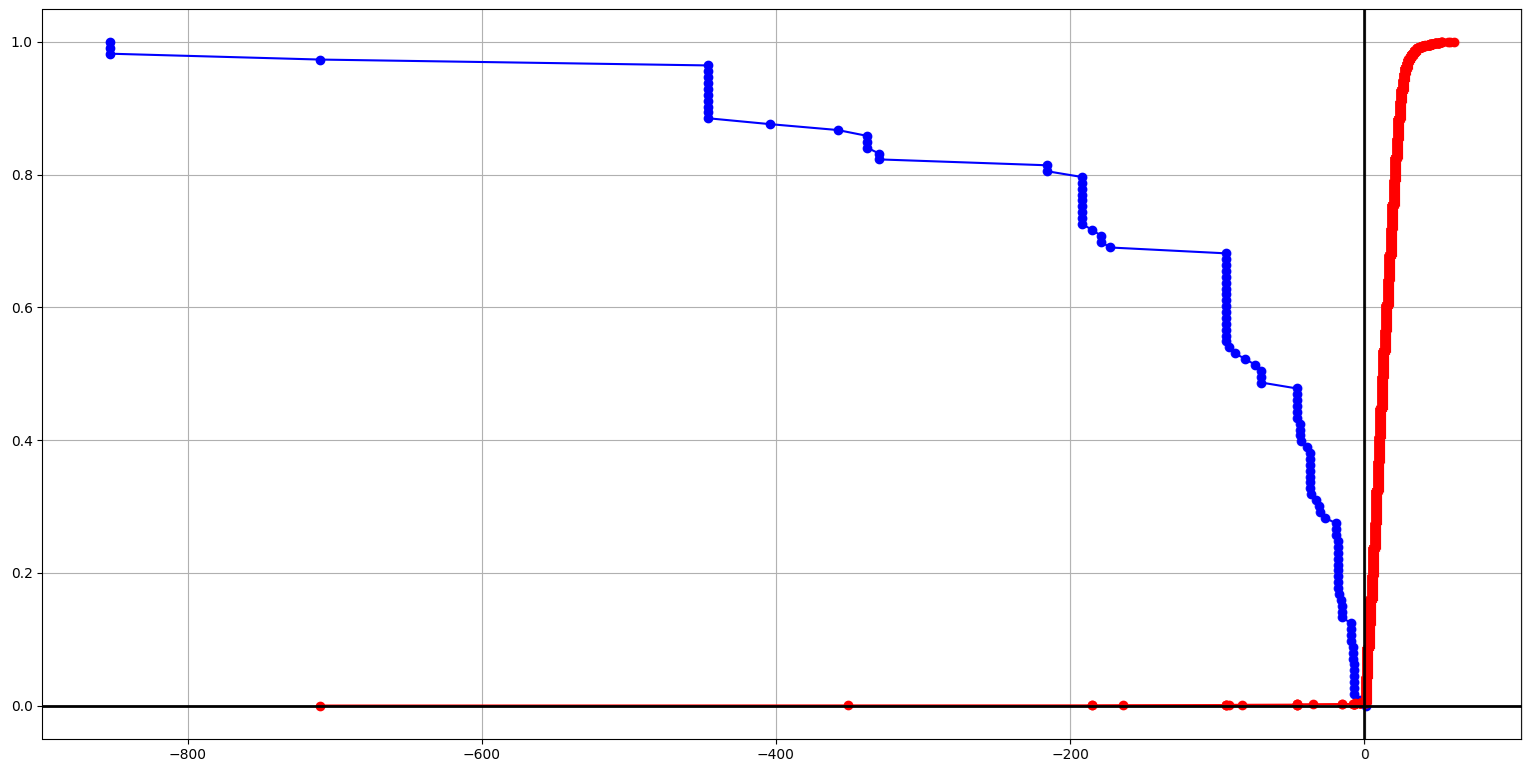
\includegraphics[width=\textwidth]{c-eval-big.png}
        \end{minipage}
        \onslide<2->{
        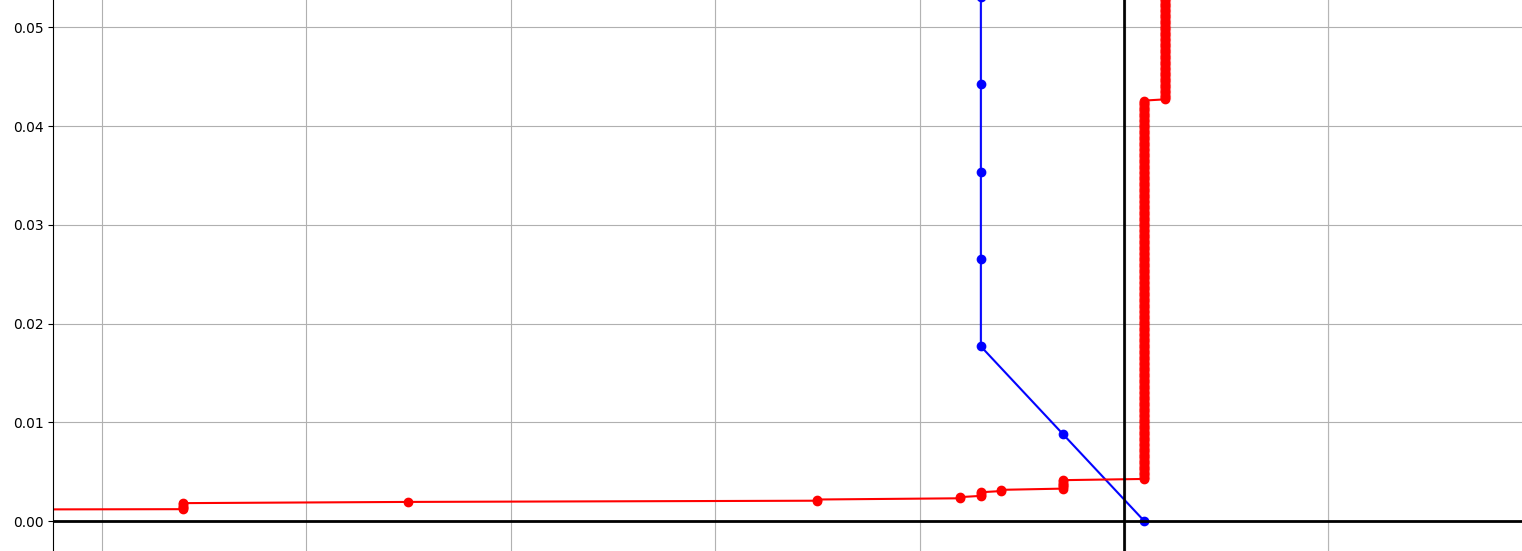
\includegraphics[width=\textwidth]{c-eval-little.png}
        }
        \vspace{-15px}
    \end{figure}
\end{frame}


\begin{frame}
    \frametitle{Experiments}
    \begin{itemize}
        \onslide<1->{
        \item WSL2 Ubuntu,
        Intel Core i7-11370H (3.30 GHz), 
        16 GB RAM} \onslide<2->{ 
        \item Apply the algorithm to the random cubic subspace instances\\
        with $\maxD=100$ and fixed $\noise=0,1,2,3,4,5$:
        \begin{itemize}
            \item 3x7 points (solve 15 instances)
            \item 3x10 points (solve 15 instances)
            \item 3x15 points (solve 7 instances)
            \item 3x20 points (solve 1 instance)
        \end{itemize}
        } \onslide<3->{
        \item Track
        \begin{itemize}
            \item computation time (s)
            \item partial optimality (\%)
            \item accuracy (\%) with respect to the truth (correct labeling)
        \end{itemize}
        } \onslide<4->{
        \item Capture
        \begin{itemize}
            \item 1.quartile (Q1)
            \item median (Q2)
            \item 3.quartile(Q3)
            \item the worst computation time
        \end{itemize}
        }
    \end{itemize}
\end{frame}


\begin{frame}
    \frametitle{Partial Optimality (3x7 points)}
    % not enough information to join all the same plane points!
    % losing partial optimality because of conflicts!
    \resizebox{0.95\textwidth}{!}{
    \begin{tikzpicture}
        \begin{axis}[
            legend style={font=\tiny},
            xlabel=$\noise$, ylabel=Partial Optimality / \%,
            grid=major,
            xmin=0, ymin=0,
            legend style={
                at={(0.35,0)},
                anchor=south east
            },
            every axis plot/.append style={line width=1.5pt}
        ]   
            \addnoiseplot{data7_of_noise.csv}{opt}{blue}
        \end{axis}
    \end{tikzpicture}
    }
\end{frame}


\begin{frame}
    \frametitle{Accuracy (3x7 points)}
    % not enough information to join all the same plane points!
    % losing partial optimality because of conflicts!
    \resizebox{0.95\textwidth}{!}{
    \begin{tikzpicture}
        \begin{axis}[
            legend style={font=\tiny},
            xlabel=$\noise$, ylabel=Accuracy / \%,
            grid=major,
            xmin=0, ymin=0,
            legend style={
                at={(0.35,0)},
                anchor=south east
            },
            every axis plot/.append style={line width=1.5pt}
        ]   
            \addnoiseplot{data7_of_noise.csv}{acc}{red}
        \end{axis}
    \end{tikzpicture}
    }
\end{frame}


\begin{frame}
    \frametitle{Partial Optimality (3x10 points)}
    % not enough information to join all the same plane points!
    % losing partial optimality because of conflicts!
    \resizebox{0.95\textwidth}{!}{
    \begin{tikzpicture}
        \begin{axis}[
            legend style={font=\tiny},
            xlabel=$\noise$, ylabel=Partial Optimality / \%,
            grid=major,
            xmin=0, ymin=0,
            legend style={
                at={(0.35,0)},
                anchor=south east
            },
            every axis plot/.append style={line width=1.5pt}
        ]   
            \addnoiseplot{data10_of_noise.csv}{opt}{blue}
        \end{axis}
    \end{tikzpicture}
    }
\end{frame}


\begin{frame}
    \frametitle{Accuracy (3x10 points)}
    % not enough information to join all the same plane points!
    % losing partial optimality because of conflicts!
    \resizebox{0.95\textwidth}{!}{
    \begin{tikzpicture}
        \begin{axis}[
            legend style={font=\tiny},
            xlabel=$\noise$, ylabel=Accuracy / \%,
            grid=major,
            xmin=0, ymin=0,
            legend style={
                at={(0.35,0)},
                anchor=south east
            },
            every axis plot/.append style={line width=1.5pt}
        ]   
            \addnoiseplot{data10_of_noise.csv}{acc}{red}
        \end{axis}
    \end{tikzpicture}
    }
\end{frame}


\begin{frame}
    \frametitle{Partial Optimality (3x15 points)}
    % not enough information to join all the same plane points!
    % losing partial optimality because of conflicts!
    \resizebox{0.95\textwidth}{!}{
    \begin{tikzpicture}
        \begin{axis}[
            legend style={font=\tiny},
            xlabel=$\noise$, ylabel=Partial Optimality / \%,
            grid=major,
            xmin=0, ymin=0,
            legend style={
                at={(0.35,0)},
                anchor=south east
            },
            every axis plot/.append style={line width=1.5pt}
        ]   
            \addnoiseplot{data15_of_noise.csv}{opt}{blue}
        \end{axis}
    \end{tikzpicture}
    }
\end{frame}


\begin{frame}
    \frametitle{Accuracy (3x15 points)}
    % not enough information to join all the same plane points!
    % losing partial optimality because of conflicts!
    \resizebox{0.95\textwidth}{!}{
    \begin{tikzpicture}
        \begin{axis}[
            legend style={font=\tiny},
            xlabel=$\noise$, ylabel=Accuracy / \%,
            grid=major,
            xmin=0, ymin=0,
            legend style={
                at={(0.35,0)},
                anchor=south east
            },
            every axis plot/.append style={line width=1.5pt}
        ]   
            \addnoiseplot{data15_of_noise.csv}{acc}{red}
        \end{axis}
    \end{tikzpicture}
    }
\end{frame}

\begin{frame}
    \frametitle{Partial Optimality}
    % 1.quartile: partial optimality loss is even more noticable
    \resizebox{0.95\textwidth}{!}{
    \begin{tikzpicture}
        \begin{axis}[
            xlabel=$\#points/3$, ylabel=Partial Optimality / \%,
            grid=major,
            xmin=6, xmax=16, ymin=0,
            legend style={
                at={(0.35,0)},
                anchor=south east
            },
            every axis plot/.append style={line width=1.5pt}
        ]   
            \addsizeplot{data_of_size.csv}{noise0}{blue}
            \addlegendentry{$\noise=0$}
            \addsizeplot{data_of_size.csv}{noise1}{orange}
            \addlegendentry{$\noise=1$}
        \end{axis}
    \end{tikzpicture}
    }
\end{frame}


\begin{frame}
    \frametitle{Partial Optimality}
    % 1.quartile: partial optimality loss is even more noticable
    \resizebox{0.95\textwidth}{!}{
    \begin{tikzpicture}
        \begin{axis}[
            xlabel=$\#points/3$, ylabel=Partial Optimality / \%,
            grid=major,
            xmin=6, xmax=16, ymin=0,
            legend style={
                at={(1,0.5)},
                anchor=south east
            },
            every axis plot/.append style={line width=1.5pt}
        ]   
            \addsizeplot{data_of_size.csv}{noise2}{green}
            \addlegendentry{$\noise=2$}
            \addsizeplot{data_of_size.csv}{noise3}{red}
            \addlegendentry{$\noise=3$}
        \end{axis}
    \end{tikzpicture}
    }
\end{frame}


\begin{frame}
    \frametitle{Computation Time (worst case)}
    % high noise => partial optimality 0
    % (all possible conditions checked at least once)
    % estimated time 1/8 * 1e-6 * (#points)^6
    % estimation: (#points)^6 / t => almost equal factors 8
    % n,time_estimated,time_worst (s)
    % 7,10.7,9
    % 10,91,93
    % 15,1038,949
    % 20,5832,5894
    % 30,66430,
    % 40,373248,
    % 50,1423828,
    \resizebox{0.95\textwidth}{!}{
    \begin{tikzpicture}
        \begin{axis}[
            legend style={font=\small},
            xlabel=\#points/3, ylabel=$\log_{10}(\text{Computation Time/s})$,
            xmin=7, xmax=30,
            xmode=log, ymode=log,
            grid=major,
            legend style={
                at={(0.95,0.05)},
                anchor=south east
            },
            every axis plot/.append style={line width=1pt}
        ]
            \addplot[color=pink, line width=4pt] table[x=n, y=time_estimated, col sep=comma] {data_time.csv};
            \addlegendentry{$\frac{1}{8}\cdot10^{-6}\cdot(\#points)^6$}
            \addplot[color=blue, mark=*, only marks, line width=2pt] table[x=n, y=time_worst, col sep=comma] {data_time.csv};
            \addlegendentry{worst computation time}
        \end{axis}
    \end{tikzpicture}
    }
\end{frame}



